\documentclass[12pt]{article}
\usepackage{amsmath,graphicx}

\title{Modeling the inductively shunted\\Cooper pair box: halfway report}
\author{John O'Connor}
\date{}

\begin{document}
\maketitle

The Cooper pair box is a well-studied quantum circuit that can be
studied as an artificial atom. The inductively-shunted Cooper pair box
(LCPB) is much less well-studied. Adding an inductive shunt promises to
reduce ambient charge noise around the circuit, but it also produces a
Hamiltonian with completely different characteristics. The first
examples of these circuits are being studied in by Vlad Manucharyan in
one of the labs in Becton. Computer models of the Hamiltonian for
these circuits exist, but they are too slow to be helpful in
interpreting the experimental data. We hope to build a more efficient
model and tools that can automatically filter those data and fit the
results.

During the first semester most of my work was geared towards learning
the physics and mathematics involved. We put together two working
models, one of a simpler potential and one of the unmodified Cooper
pair box. I used the latter to produce the energy graphs I showed in my
presentation. We also coded a filter to pull relevant curves out of
our experimental data.

\begin{center}
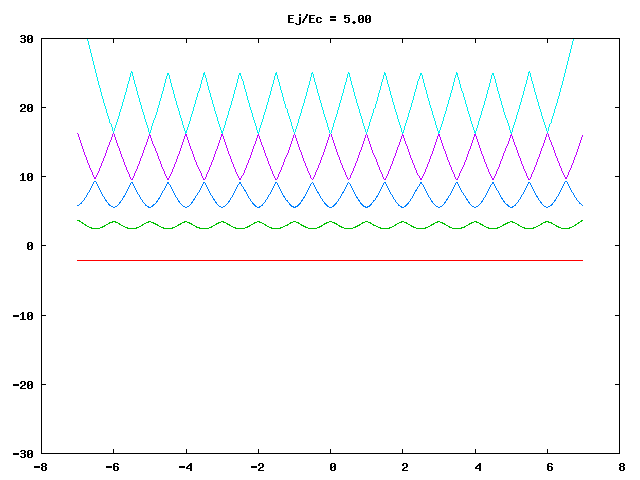
\includegraphics[scale=0.33]{parabolas.png}\\
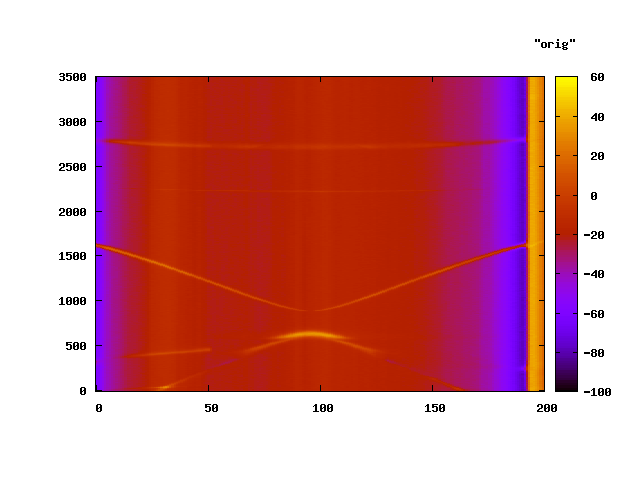
\includegraphics[scale=0.30]{orig.png}
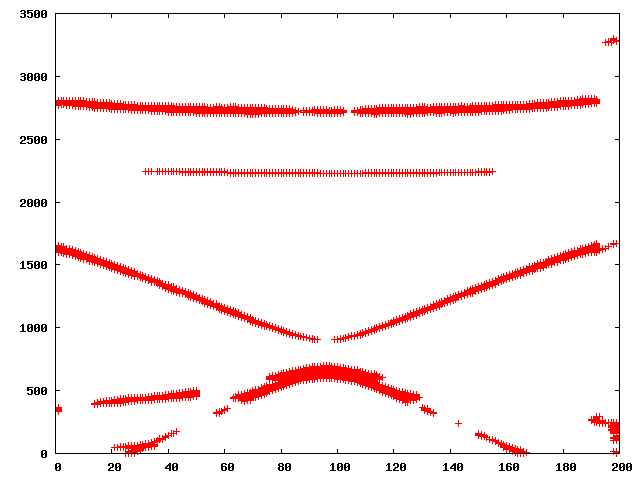
\includegraphics[scale=0.30]{pic.png}
\end{center}

In the second semester, the main focus will be on adapting the
previous semester's work to the LCPB. Once that is working, the
biggest challenge will be to put together automatic curve fitting for
the experimental data. That will be the point where the inefficiencies
of our model begin to show. Once everything is working, we should be
able to get a better handle on our existing experimental data and
guide the experiments into new parameter regimes.

All of the work so far has been done in the Python programming
language, using a library called SciPy for the higher mathematics
(Hermite polynomials and linear algebra). Python is an excellent
environment for prototyping, but one possibility moving forwards,
after we finish the first version of our final product, will be to
look for less convenient but more efficient alternatives. One of the
biggest factors slowing down existing models in Mathematica is
arithmetic performed on extremely large and extremely small floating
point numbers. Coding the bignum arithmetic ``by hand'' might give us
more flexibility to make approximations, if we ultimately have enough
time to implement that.

\end{document}
